\subsection{Kubernetes at the Edge}

\begin{flushleft}
The below diagram shows the architecture of Kubeedge project, an initiative to develop Edge platform using Kubernetes. The details about the project and its source can be found in \cite{kedge}.
\end{flushleft}

\begin{figure}[h!]
    \centering
    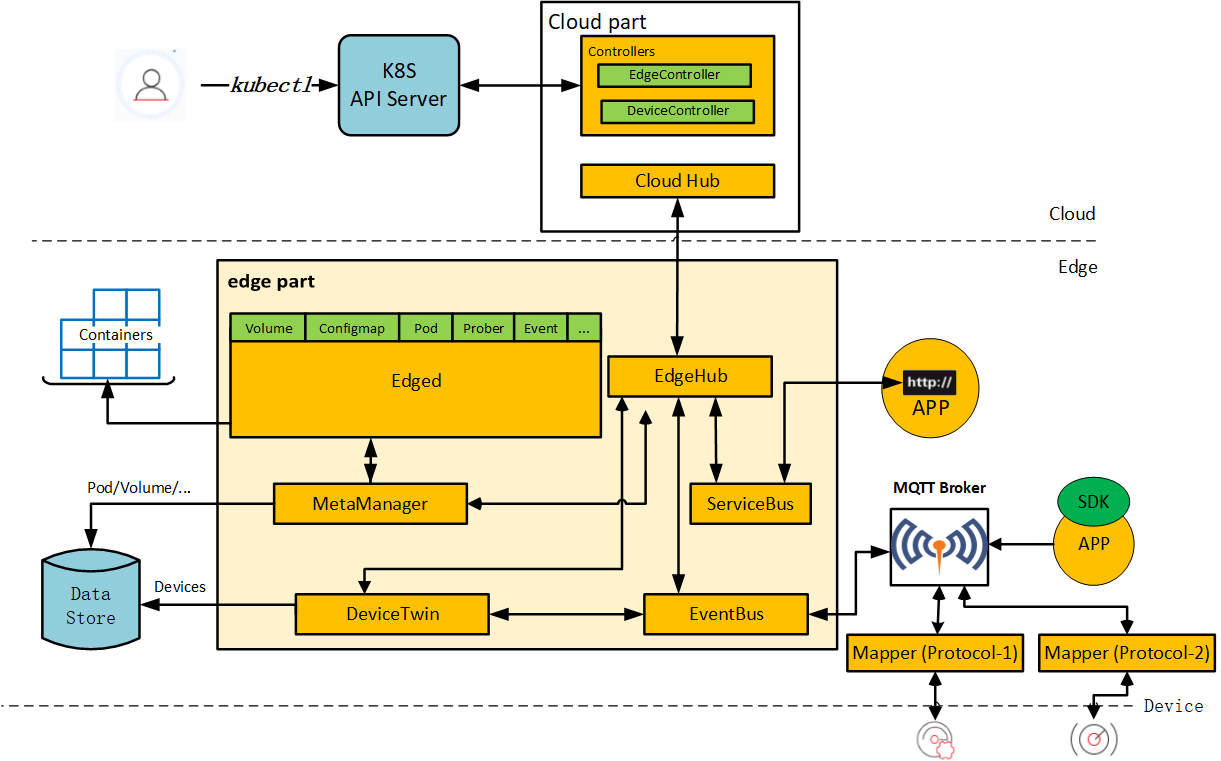
\includegraphics[width=0.9\textwidth]{k8s_edge}
    \label{fig:figure14}
	\caption{Architecture of the KubeEdge project. From \cite[What is KubeEdge]{kedgedoc}}
\end{figure}

\begin{flushleft}
The architecture as shown in Figure 14 consists of two parts:
\end{flushleft}
\begin{enumerate}
    \item \textbf{The Cloud Part}
	    The components that run in the data center and provides mechanisms for the edge part to synchronize with the cloud part. The cloud part consists of the following components:
        \begin{itemize}
            \item \textit{Edge Controller:} - interfaces with the Kubernetes API Server and syncs with the events and updates with the edge core.
            \item \textit{Device Controller:} - Updates and syncs device status using device model and device instance. 
            \item \textit{Cloud Hub:} - Prepares the platform for communication between the cloud and the edge (websocket, channelQ, messages)
		\end{itemize}
    \item \textbf{The Edge Part}
        The components that run on the edge device and interact with the end-user equipment. It synchronizes with the cloud part for functions like device management and service updates. It comprises the following components:
		\begin{itemize}
            \item \textit{EdgeD:} - A daemon that manages the life cycle of the pod/s on the edge node. It proposes to include a CRI as a replacement for the current docker runtime to ensure a lightweight runtime and also provide options to choose from multiple container runtimes.
            \item \textit{EventBus:} - Is responsible for sending/receiving messages over MQTT to/from external clients.
            \item \textit{MetaManager:} - Responsible to process, store and query messages between the Edgehub and the EdgeD. 
            \item \textit{Edgehub:} - Interacts with the Cloud Hub on the cloud part either through web-socket or using QUIC protocol. The functions include reporting device and edged status to the cloud and sync with cloud-side resources.
            \item \textit{DeviceTwin:} - Supports Device management through storing and querying device status, health check, message distribution and membership management.
	    \end{itemize}
\end{enumerate}
